\chapter{Release Management}
\section{Aufgaben und funktionale Einordnung}
Das Release Management ist für die effektive, sichere und nachvollziehbare Durchführung von Änderungen der IT-Infrastruktur verantwortlich. Aufgaben des Release Managements sind die Planung, Überwachung und Durchführung von Rollouts und Rollins. Dies erfolgt in Abstimmung mit dem Change Management.  Ferner hat das Release Management die Aufgabe die Gesamtheit der Änderungen der IT zeitlich, technisch und inhaltlich zu bündeln und aufeinander abzustimmen. \cite{wiki-it}, \cite{rm-pilorget}
\\
Die Funktion des Release Management ist dem Service Support zugeordnet. Dieser hat die operativen Prozesse zur Behandlung von Service-Unterbrechungen und Durchführung zur Aufgabe und garantiert somit die Aufrechterhaltung der IT-Services. Der Service Support ist wiederum dem IT Service Management zugeordnet.  \cite{wiki-it-service}

\section{Einteilung von Releases}
\textbf{Emergency Release:}
\\
Behebung von Störungen oder signifikanten Problemen in der IT. Ähnelt dem Minor Release, benötigt jedoch \acs{i.d.R.} viel weniger Zeit.
\\
\textbf{Minor Release:}
\\
Dieser Release enthält kleinere Erweiterungen und Fixes. Werden häufiger als Major Releases durchgeführt, benötigen jedoch weniger Zeit und Planung. Ersetzen voran-gegangene Emergency Releases. 
\\
\textbf{Major Release:}
\\
Beinhaltet signifikante neue Funktionalitäten, Upgrades, oder neue Services in der IT. Ersetzen alle vorangegangen Minor und Emergency Releases, welche bezüglich eines Problems in der IT durchgeführt wurden und macht diese überflüssig. Dieser Release wird selten durchgeführt, benötigt jedoch mehr Zeit und Planung als Minor und Emergency Releases.
\cite{rm-howard}
\section{Teilprozesse}
Die Teilprozesse des Release Management nach ITIL sind in der folgenden Abbildung \ref{fig:tp} dargestellt. 
\begin{figure}[H]
	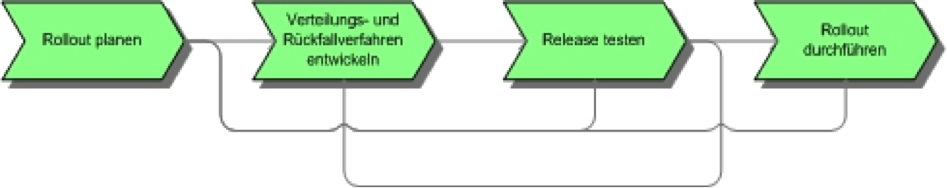
\includegraphics[width=\textwidth]{img/Teilprozesse.png}
	\caption{Teilprozesse des Release Management nach ITIL \cite{wiki-it}}
	\label{fig:tp}
\end{figure}
\textbf{Rollout planen:}
\\
Für die Planung eines Release wird eine Vielzahl von Informationen benötigt. Diese sind in einem Release-Plan und einem Release-Steckbrief gebündelt. \cite{rm-schiefer-erik}
\\
\textbf{Release-Plan:}
\begin{itemize}
	\item Abstimmung über den Inhalt des Releases
	\item Absprache über zeitliche Reihenfolge, Standorte und Organisationsbereiche
	\item Klärung der eingesetzten Hard- und Software
	\item Klärung der erforderlichen Mittel für Hardware, Software und Dienstleistungen
	\item Abstimmung der Verantwortlichen
	\item Dienstleistungen, welche von Dritten benötigt und über das Supplier Management koordiniert werden
	\item Erstellen von Back-Out-Plänen
	\item Aufwandsabschätzung
\end{itemize}
\textbf{Release-Steckbrief:}
\begin{itemize}
	\item Name des Release
	\item Version des Release
	\item Beschreibung des Release
	\item Dokumentationsablage
	\item Historie
\end{itemize}


\textbf{Verteilungs- und Rückfallverfahren entwickeln:}
\\
In diesem Teilprozess werden die technischen Voraussetzungen zur Installation, bzw. der Verteilung der neuen Komponenten des Release geschaffen. Des Weiteren werden hier Vorkehrungen für das Zurückfahren des Rollouts für den Fall von unvorhergesehenen Problemen getroffen. \cite{wiki-it}
\\
\textbf{Release testen:}
\\
Der Test des Release erfolgt in der Regel durch das Betriebspersonal (=> Realitätsnähe). Besonderer Beachtung sollten hierbei der Funktionsweise, den technischen Betriebs-aspekten, dem Leistungsverhalten und der Integration in die vorhandene Infrastruktur geschenkt werden.  
\cite{rm-schiefer-erik}
\\
Im Rahmen des Release Prozesses sind drei Arten von Tests vorgesehen. Dies sind der Unit-, Integration- und der Abnahme-Test. \cite{rm-pilorget} 
\\
Für den Unit-Test ist der Applikationsexperte verantwortlich. Hierbei wird geprüft, ob jedes Element des Release so funktioniert, wie es spezifiziert wurde. Es werden Testprogramme und Testskripte geschrieben. Hierbei werden einfache Testfälle benutzt. 
Die Verantwortung für den Integration Test trägt der IT-Projektleiter. Dieser überprüft, ob die definierten Funktionen und Schnittstellen funktionieren und im Verbund funktionieren. Hierbei sollen möglichst alle Benutzer-Szenarien berücksichtigt werden. 
Für den Abnahme-Test ist der Fachprojektleiter verantwortlich. Dieser Test unterteilt sich in einen User Acceptance Test und einen Regression Test. Im User Acceptance Test wird geprüft, ob das System alle geforderten Business-Funktionalitäten abdeckt und den korrekten Output generiert. Im Regression Test wird sichergestellt, dass die System-veränderungen nicht einen vorher funktionierenden Systemteil beeinflusst haben. 
\\
\textbf{Rollout durchführen:}
\\
Dieser Prozess hat einerseits zum Ziel, die Release-Komponenten in die IT-Umgebung auszurollen. D.h. die neuen Funktionalitäten werden auf alle Zielobjekte ausgebreitet und installiert. Die Mitarbeiter, welche von den Änderungen der Releases betroffen sind, werden geschult. Die Dokumentation über entsprechende Konfigurationselemente wird aktualisiert. 
\cite{rm-pilorget}
\\ 
Andererseits findet eine Erfolgskontrolle statt. \cite{wiki-it}
